\documentclass[a4paper, 12pt, ngerman]{exam}
\usepackage{preamble/draft}
%\usepackage{polynom}
\usepackage{pgfplots}
\pgfplotsset{compat = newest}

% layout for listings
\lstset{
 morekeywords={for, in, if, then, endfor},
 basicstyle=\ttfamily,
 keywordstyle=\bfseries,
 frame=single,
 frameround=tttt,
 escapeinside={|}{|},
 numbers=left,
 numberstyle=\tiny,
 breaklines=true
}

% page layout
\geometry{a4paper,left=2.5cm,right=2.5cm, top=3cm, bottom=3cm}

% font layout
\titleformat{\chapter}[display]
  {\normalfont\sffamily\huge\bfseries}
    {\chaptertitlename\ \thechapter}{20pt}{\Huge}
%\titleformat*{\chapter}{\LARGE\bfseries\sffamily}
\titleformat*{\section}{\Large\bfseries\sffamily}
\titleformat*{\subsection}{\large\bfseries\sffamily}
\titleformat*{\subsubsection}{\normalsize\bfseries\sffamily}
\titleformat*{\paragraph}{\small\bfseries\sffamily}
\titleformat*{\subparagraph}{\footnotesize\bfseries\sffamily}



\newcommand{\examtype}{Übung Differentialrechnung}
\newcommand{\examno}{2}
\newcommand{\examdate}{26.04.2022}
\newcommand{\subject}{Mathematik}
\newcommand{\examclass}{}

%\addpoints
\pointpoints{Punkt}{Punkte}
\bonuspointpoints{Bonuspunkt}{Bonuspunkte}
\renewcommand{\solutiontitle}{\noindent\textbf{Lösung:}%
\enspace}

\chqword{Frage}
\chpgword{Seite}
\chpword{Punkte}
\chbpword{Bonuspunkte}
\chsword{Erreicht}
\chtword{Gesamt}

\hpword{Punkte:} % Punktetabelle
\hsword{Ergebnis:}
\hqword{Aufgabe:}
\htword{Summe:}

\pagestyle{headandfoot}
\firstpageheadrule
\runningheadrule
\firstpageheader{\examclass}{\large{\textbf{\subject}}\\ \large{\examtype\ \examno}}{\examdate}
\runningheader{\examclass}{\large{\textbf{\subject}}\\ \large{\examtype\ \examno}}{\examdate}
\firstpagefooter{}{Seite \thepage\ von \numpages}{}
\runningfooter{}{Seite \thepage\ von \numpages}{}

\qformat{\textbf{Aufgabe \thequestion} \hfill}
\pointformat{}

\pointsinrightmargin

\renewcommand{\familydefault}{\sfdefault}

\colorgrids
\definecolor{GridColor}{gray}{0.7}

\tikzumlset{fill class=white}


%\printanswers

\begin{document}

\begin{questions}
 
  \question
  Gegeben sei folgender Graph der Funktion $f(x) = x^3+2x^2-5$:
  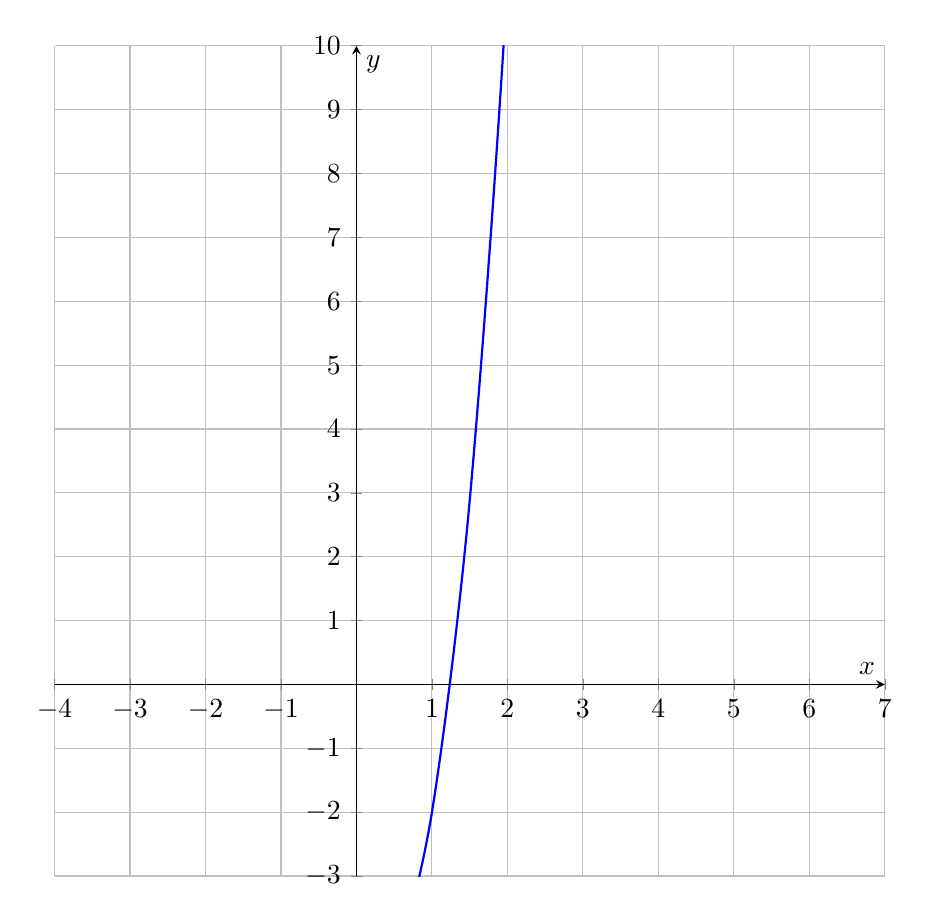
\begin{tikzpicture}
    \begin{axis}[
        xmin = -4.0, xmax = 7.0,
        ymin = -3.0, ymax = 10.0,
        xtick distance = 1.0,
        ytick distance = 1.0,
        major grid style = {lightgray},
        minor grid style = {lightgray!25},
        grid = both,
        width = \textwidth,
        height = \textwidth,
        axis x line=center,
        axis y line=center,
        xlabel = {$x$},
        ylabel = {$y$},
      ]
        \addplot[
            domain = -4:8,
            smooth,
            thick,
            blue,
        ] {x^3+2*x^2-5};
    \end{axis}
    \end{tikzpicture}
  \begin{parts}
    \part
    \begin{solution}
    \end{solution}
  \end{parts}

\end{questions}

\end{document}
